\maketitle
\tableofcontents
\newpage

\section{Zielsetzung}
In diesem Versuch wird die Fourier-Analyse und -Synthese untersucht. Dabei werden
aus Fourier-Komponenten Schwingungen moduliert und bekannte Schwingungen in selbige
zerlegt.

\section{Theorie}
Eine wichtige Rolle beim Fourier-Formalismus spielen periodische Funktionen.
Diese sind definiert durch
\begin{align*}
      f(t + T) &= f(t) \ \text{für zeitliche Periodizität} \\
      f(x + D) &= f(x) \ \text{für räumliche Periodizität} \, .
\end{align*}
Dabei ist $T$ bzw. $D$ die Periodendauer der Funktion; also der Zeitraum,
nachdem $f(t)$ bzw. $f(x)$ wieder den gleichen Wert wie bei $t$ bzw. $x$ hat.
Dafür bieten sich die Sinus- und Cosinus-Funktion an.
Sie finden sich in dem sogennanten Fourierschem Theorem
\begin{equation}
    f(t) = \frac{1}{2} a_0 + \sum_{n = 1}^{\infty} \left(a_n \, \symup{cos} \left(n \frac{2\pi}{T} t \right)
    + b_n \, \symup{sin} \left(n \frac{2\pi}{T} t \right) \right)
    \label{eqn:1}
\end{equation}
wieder, welches erfüllt ist, falls die Reihe aus \eqref{eqn:1} gleichmäßig konvergiert.
Dann gilt für die Koeffizienten $a_n$ und $b_n$
\begin{align}
    a_n &= \frac{2}{T} \int_0^T f(t) \, \symup{cos} \left(n \frac{2\pi}{T} t \right) \symup dt
    \label{eqn:2} \\
    b_n &= \frac{2}{T} \int_0^T f(t) \, \symup{sin} \left(n \frac{2\pi}{T} t \right) \symup dt
    \label{eqn:3}
\end{align}
mit $n \in \mathbb{N}$. An \eqref{eqn:2} und \eqref{eqn:3} sieht man, dass in \eqref{eqn:1} nur ganzzahlige
Vielfache der Grundfrequenz $\nu_1 = \frac{1}{T}$ auftreten. Die Ermittlung der Größen
$a_n$ und $b_n$ nennt man Fourier-Analyse. Wenn man \eqref{eqn:2} und \eqref{eqn:3} gegen
die Frequenz aufträgt, erhält man ein Linienspektrum, wie in Abbildung \ref{fig:1} zu sehen.
\begin{figure}
  \centering
  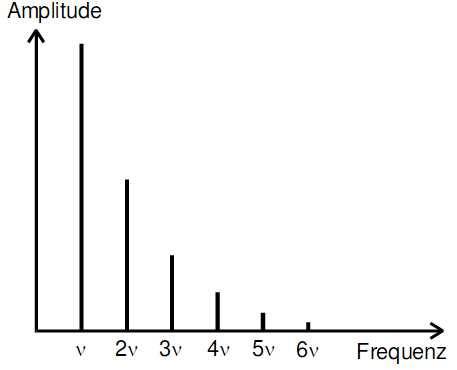
\includegraphics[scale=0.4]{spektrum.png}
  \caption{Linienspektrum einer periodischen Funktion mit Grundfrequenz $\nu$.}
  \label{fig:1}
\end{figure}
Falls $f(t)$ an einer Stelle $t_0$ nicht stetig sein sollte, dann konvergiert \eqref{eqn:1} nicht gleichmäßig
und es tritt eine endliche Abweichung in $f(t_0)$ auf. Diese Abweichung wird für
$n \to \infty$ im Gegensatz zu \eqref{eqn:2} und \eqref{eqn:3} nicht kleiner, sodass sie
in diesem Experiment gut zu beobachten ist, da es sich um Fouriersummen handelt. Die oben
beschriebene Abweichung nennt man Gibbsches Phänomen.

Mit der Fourier-Transformation
\begin{equation}
    g(\nu) = \int_{- \infty}^{\infty} f(t) \, e^{i\nu t} \, \symup dt
    \label{eqn:4}
\end{equation}
lässt sich das ganze Frequenzspektrum $g(\nu)$ einer Funktion $f(t)$ bestimmen,
egal ob sie periodisch ist oder nicht. Falls $f(t)$ periodisch ist, ergibt sich aus
\eqref{eqn:4} eine Reihe aus $\delta$-Distributionen; falls $f(t)$ nicht-periodisch ist,
ist das Frequenzspektrum kontinuierlich. Da es im Experiment nicht möglich ist über
einen unendlichen langen Zeitraum (wie in \eqref{eqn:4} gefordert) zu integrieren,
ergibt sich für jede Funktion $f(t)$ ein kontinuierliches Spektrum. Außerdem werden
Nebenmaxima entstehen, die in der Auswertung gefiltert werden müssen.

\section{Durchführung}

\subsection{Versuchsaufbau}

\subsection{Versuchsdurchführung}

\section{Auswertung}

\section{Diskussion}
\newpage
\nocite{*}
\printbibliography
